% GENERATED by implementation/experiments/scripts/render_v005_figures.py.
% Do not edit by hand -- regenerate from results/runs/<root>/ instead.

\begin{figure*}[t]
    \centering
    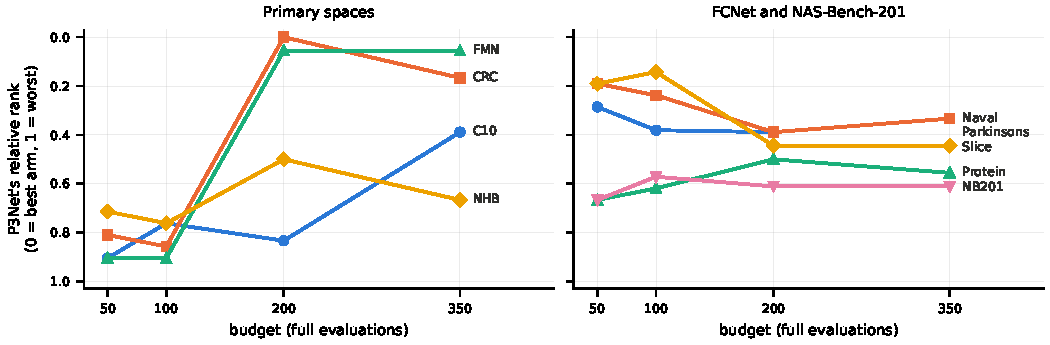
\includegraphics[width=\textwidth]{figures/rank__p3net__by_budget.pdf}
    \caption{P3Net's standing by budget: relative rank of its median final quality among the main-track arms run in the cell (0 = best, 1 = worst; 22 arms at $b \le 100$, 19 at $b \ge 200$, ties share the lower rank). Left: the primary spaces; right: the FCNet tasks and NAS-Bench-201.}
    \Description{Two line charts of P3Net's relative rank against the budget, one line per search space: on most spaces the rank improves from near the worst at 50 evaluations to near the best at 200 or 350.}
    \label{fig:v005-rank-budget}
\end{figure*}

\begin{figure*}[t]
    \centering
    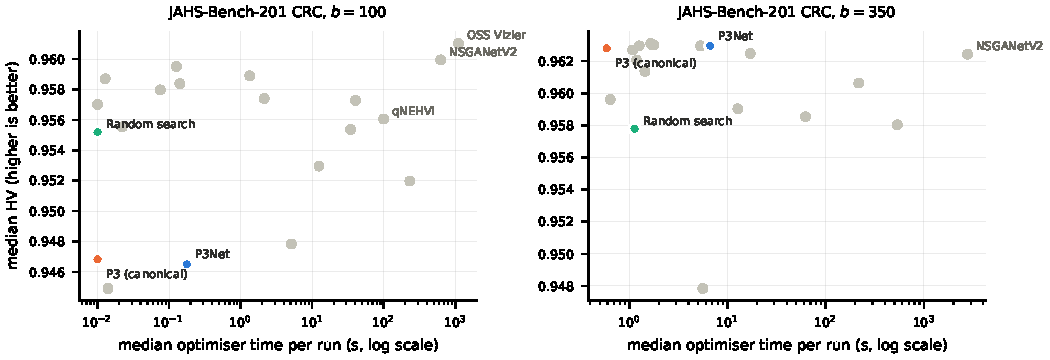
\includegraphics[width=\textwidth]{figures/quality_vs_cost__colorectal.pdf}
    \caption{Quality against the optimiser's own cost on JAHS-Bench-201 Colorectal Histology: median HV over 30 seeds and median optimiser wall-clock time per run without benchmark queries (log scale), one point per main-track arm, at $b = 100$ (with the Gaussian-process arms) and $b = 350$; times below 0.01\,s are drawn at 0.01\,s. Coloured: P3Net, canonical P3 and random search; grey: the other arms.}
    \Description{Two scatter plots of median hypervolume against optimiser time on a log axis; the Gaussian-process arms and NSGANetV2 are the most expensive, P3Net and canonical P3 among the cheapest.}
    \label{fig:v005-quality-cost}
\end{figure*}

\begin{figure}[t]
    \centering
    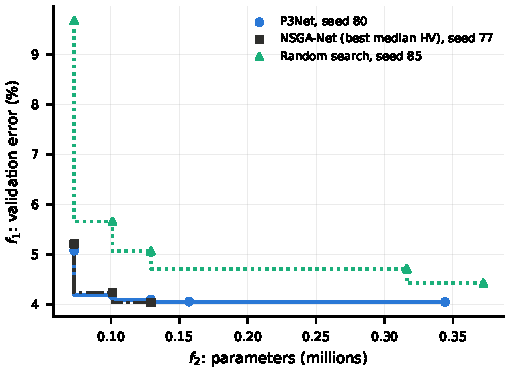
\includegraphics[width=\linewidth]{figures/fronts__colorectal__budget350.pdf}
    \caption{Final non-dominated fronts of the median run (by HV) of P3Net, of the arm with the best median HV (NSGA-Net) and of random search, JAHS-Bench-201 Colorectal Histology, $b = 350$; both objectives are minimised.}
    \Description{Step plots of validation error against parameter count for three fronts; the fronts of P3Net and of the best arm both reach about four percent error, random search's front stays higher.}
    \label{fig:v005-fronts}
\end{figure}
